% ================================================================
\section{Preliminary Results}\label{sec:experiments}

We validate the proposed methods in simulation using
a Crazyflie 2.1 quadrotor model (mass 35\,g, arm length 46\,mm)
with a control frequency of 50\,Hz.
All simulations use a Python reference implementation
with NumPy linear algebra.

\subsection{Controller Variants}

Across the three experiments we use up to five controller variants.
The hover and figure-eight experiments compare four:
\begin{enumerate}
  \item \textbf{TinyMPC} (baseline): Fixed linearization at hover,
    ADMM with warm-starting and convergence tolerance $10^{-3}$.
  \item \textbf{Online Relinearization}: Autograd-based Jacobian
    at each timestep, fresh DARE solve, then ADMM.
  \item \textbf{Flat Template MPC}: $\balpha$-parameterized analytic
    linearization with precomputed DARE cache grid, then ADMM.
  \item \textbf{Analytic Template}: Zero-iteration state feedback
    with first-order gain interpolation.
\end{enumerate}
The circle-in-square experiment (Section~\ref{sec:circle_square})
replaces TinyMPC with:
\begin{enumerate}
  \setcounter{enumi}{4}
  \item \textbf{Barrier Template}: Zero-iteration state feedback
    with barrier-augmented DARE cache (Section~\ref{sec:barrier}),
    providing soft constraint awareness at ${\sim}260$ operations.
\end{enumerate}

\subsection{Hover Stabilization}

The quadrotor starts at $(0.2, 0.2, -0.2)$\,m from the hover point.
Horizon $N=10$, penalty $\rho = 85$, $N_{\mathrm{sim}} = 100$ steps.

\begin{table}[t]
\centering
\caption{Hover stabilization ($N_{\mathrm{sim}}=100$, $\rho=85$, $N=10$).}
\label{tab:hover}
\begin{tabular}{@{}lcccc@{}}
\toprule
 & Tiny & Online & Flat & Analytic \\
 & MPC & Relin & Template & Template \\
\midrule
Avg.\ pos.\ error (m)  & \textbf{0.064} & 0.095 & 0.138 & 0.145 \\
Max pos.\ error (m)    & 0.346 & 0.346 & 0.346 & 0.346 \\
Avg.\ ADMM iters       & 80.0 & 16.7 & 7.8 & 0 \\
Total ADMM iters       & 8002 & 1669 & 785 & 0 \\
Wall time (s)          & 2.85 & 12.13 & \textbf{0.44} & \textbf{0.13} \\
\bottomrule
\end{tabular}
\end{table}

At hover, TinyMPC's fixed linearization is exact and achieves the
lowest average error (Table~\ref{tab:hover}, Fig.~\ref{fig:hover}).
However, it requires $10\times$ more ADMM iterations than the
Flat Template due to the high $\rho$ value.
The Flat Template converges faster because its cache already
incorporates the correct equilibrium structure.
The Analytic Template achieves the lowest wall-clock time
($22\times$ faster than TinyMPC) at a modest accuracy penalty.

\begin{figure}[t]
  \centering
  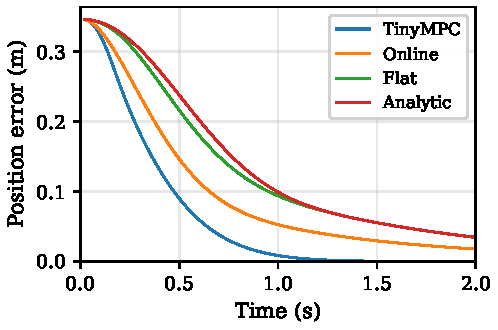
\includegraphics[width=\columnwidth]{figures/fig_hover.pdf}
  \caption{Hover stabilization: position error over time for all
    four variants. Initial displacement $(0.2, 0.2, -0.2)$\,m.
    All variants converge; the flat-parameterized controllers
    trade slightly slower convergence for significantly lower
    computation per step.}
  \label{fig:hover}
\end{figure}

\subsection{Figure-Eight Trajectory Tracking}

The reference is a figure-eight in the $xz$-plane with amplitude 0.5\,m
and period 3.7\,s.
Horizon $N=15$, penalty $\rho = 5$, $N_{\mathrm{sim}} = 200$ steps.
The Flat Template uses 21 cache entries sampled uniformly over one period.

\begin{table}[t]
\centering
\caption{Figure-eight trajectory tracking ($N_{\mathrm{sim}}=200$, $\rho=5$, $N=15$).}
\label{tab:traj}
\begin{tabular}{@{}lcccc@{}}
\toprule
 & Tiny & Online & Flat & Analytic \\
 & MPC & Relin & Template & Template \\
\midrule
Avg.\ pos.\ error (m)  & \textbf{0.033} & 0.035 & 0.035 & 0.036 \\
Max pos.\ error (m)    & \textbf{0.091} & 0.092 & 0.113 & 0.116 \\
Avg.\ ADMM iters       & 8.0 & 5.1 & 3.6 & 0 \\
Total ADMM iters       & 1598 & 1023 & 714 & 0 \\
Wall time (s)          & 1.16 & 22.02 & 0.75 & \textbf{0.26} \\
\bottomrule
\end{tabular}
\end{table}

\begin{figure}[t]
  \centering
  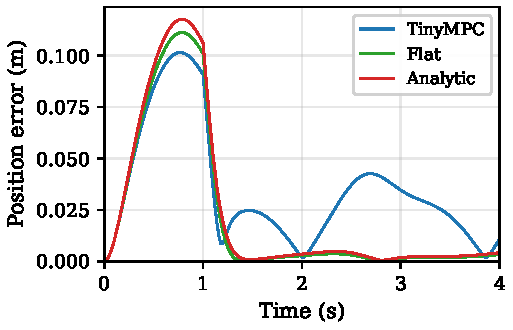
\includegraphics[width=\columnwidth]{figures/fig_traj_error.pdf}
  \caption{Figure-eight tracking: position error over time.
    All variants achieve comparable accuracy;
    the periodic structure reflects the trajectory curvature.}
  \label{fig:traj_error}
\end{figure}

\begin{figure}[t]
  \centering
  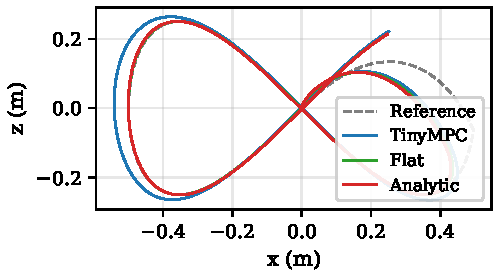
\includegraphics[width=\columnwidth]{figures/fig_traj_xz.pdf}
  \caption{Figure-eight tracking: $x$--$z$ plane view.
    The Flat Template and Analytic Template closely follow
    the reference trajectory (dashed), comparable to TinyMPC.}
  \label{fig:traj_xz}
\end{figure}

On the figure-eight trajectory (Table~\ref{tab:traj},
Figs.~\ref{fig:traj_error}--\ref{fig:traj_xz}),
all four variants
achieve similar average tracking errors ($0.033$--$0.036$\,m),
demonstrating that the flat-parameterized linearization is sufficiently
accurate for moderate-aggressiveness trajectories.
The key differences are computational:
\begin{itemize}
  \item The Flat Template requires $55\%$ fewer total ADMM iterations
    than TinyMPC and runs $1.5\times$ faster in wall-clock time.
  \item Online relinearization is $29\times$ slower than the
    Flat Template due to per-step autograd Jacobian evaluation and
    DARE solves, despite using fewer ADMM iterations.
  \item The Analytic Template achieves $4.5\times$ speedup over
    TinyMPC with only 0.003\,m additional average error, using
    \emph{zero} ADMM iterations.
\end{itemize}

\subsection{Circle-in-Square Constrained Tracking}\label{sec:circle_square}

To demonstrate the complexity cascade, we track a circular
trajectory in the $xy$-plane ($R = 0.3$\,m, period 8\,s)
while enforcing square position bounds
$|x| \leq L$, $|y| \leq L$
with $L = R / \sqrt{2} \approx 0.212$\,m, so that the
four vertices of the square lie \emph{exactly} on the circle
(inscribed square geometry; see Fig.~\ref{fig:circle_square}).
At the cardinal points, the circle exceeds the square by
$R - L \approx 88$\,mm.

We compare all four controller variants.
The Online Relinearization and Flat Template both use ADMM
with per-step horizon bounds: at horizon step $j$, the
error-state position constraint is
$-L - p_{\mathrm{ref}}(t{+}j\Delta t)
 \leq \delta x_{0:2}
 \leq L - p_{\mathrm{ref}}(t{+}j\Delta t)$,
correctly mapping the absolute constraint to error coordinates
at each future timestep.
The Barrier Template absorbs position-constraint awareness into
$Q_\mu$ via~\eqref{eq:barrier_hess_x}--\eqref{eq:Q_barrier}.
The Analytic Template tracks the full circle without constraints.
Parameters: $N = 20$, $\rho = 50$, up to 500 ADMM iterations
(for ADMM variants).

\begin{table}[t]
\centering
\caption{Circle-in-square tracking
  ($R=0.3$\,m, $L=R/\sqrt{2}$, period 8\,s).
  Moving down the cascade trades constraint fidelity for
  real-time guarantees.}
\label{tab:circle}
\begin{tabular}{@{}lcccc@{}}
\toprule
 & Online & Flat Templ. & Barrier & Analytic \\
 & Relin & (ADMM) & (zero-iter) & (zero-iter) \\
\midrule
Complexity & $O(n^3{+}Kn^2)$ & $K{\cdot}O(n^2)$ & $O(nm)$ & $O(nm)$ \\
Constraints & Hard & Hard & Soft & Clip \\
Avg.\ pos.\ err (m) & 0.062 & 0.062 & 0.017 & 0.017 \\
Max viol.\ (mm) & 0.0 & 0.0 & 88.4 & 88.4 \\
Mean viol.\ (mm) & 0.0 & 0.0 & 45.8 & 45.7 \\
Avg.\ ADMM iters & 450.8 & 450.8 & 0 & 0 \\
Wall time (s) & 168.1 & 157.4 & 0.65 & 0.62 \\
\bottomrule
\end{tabular}
\end{table}

\begin{figure}[t]
  \centering
  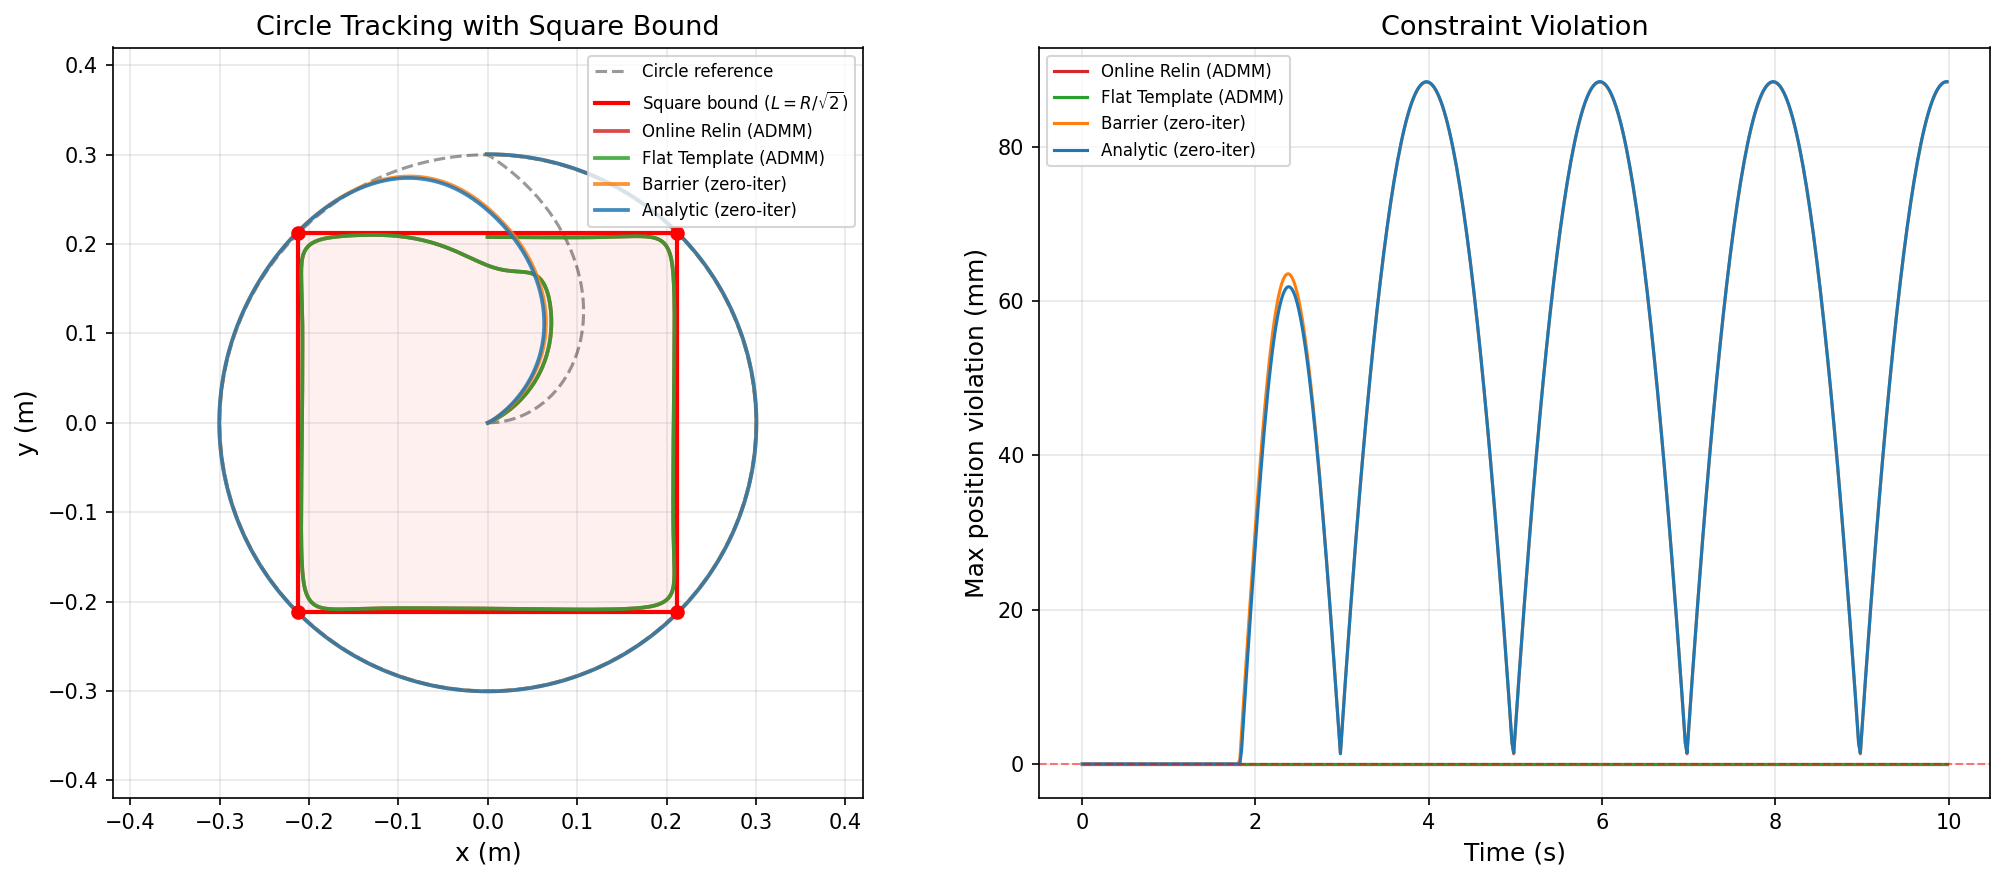
\includegraphics[width=\columnwidth]{figures/fig_circle_square.png}
  \caption{Circle-in-square constrained tracking:
    the complexity cascade from $O(n^3)$ online NMPC
    to $O(n{\cdot}m)$ deterministic feedback.
    \textbf{Left:} $xy$-plane trajectories.
    Online Relin and Flat Template (ADMM) are visibly
    ``pinched'' toward the square at the cardinal points;
    both zero-iteration variants (Barrier and Analytic)
    track the full circle with identical 88\,mm violation,
    confirming that the barrier Hessian cannot override
    a reference that lies outside the feasible region.
    \textbf{Right:} Position violation over time,
    illustrating the constraint-fidelity/computation tradeoff.}
  \label{fig:circle_square}
\end{figure}

Table~\ref{tab:circle} and Fig.~\ref{fig:circle_square}
illustrate the central tradeoff of the
hierarchy~\eqref{eq:full_chain}.
The two ADMM variants (Online Relinearization and Flat Template)
achieve near-zero position violation by encoding the absolute
constraint as per-step error-state bounds along the prediction
horizon, actively projecting the trajectory onto the feasible
set at each ADMM iteration.
The Flat Template achieves the same constraint satisfaction
as Online Relinearization while eliminating the per-step
DARE solve.

The zero-iteration variants (Barrier and Analytic) exhibit
the full geometric violation of $R - L = 88$\,mm.
This is expected: the barrier Hessian~\eqref{eq:barrier_hess_x}
penalizes error-state excursions from the reference, but in
this geometry the \emph{reference itself} exceeds the square
boundary at the cardinal points ($R > L$).
No modification of the error-state cost can prevent absolute
position violation when the tracking target lies outside the
feasible region---only the ADMM projection (which maps
absolute bounds to per-step error-state bounds) can achieve this.
The barrier remains effective for \emph{input} constraints
(preventing motor saturation) and for state constraints where
the reference stays inside the feasible region.

The key message: \emph{moving down the cascade trades constraint
fidelity for real-time guarantees}.
The ADMM variants handle arbitrary absolute constraints via
iterative projection at $O(n^2)$ per iteration;
the zero-iteration variants achieve deterministic $O(n{\cdot}m)$
feedback (${\sim}260$ operations) enabled by the
flatness-compressed $\R^4$ scheduling space, at the cost of
relinquishing hard state-constraint satisfaction.

\subsection{Numerical Validation}

We verify the implementation with four tests:
\begin{enumerate}
  \item \textbf{Linearization consistency}: At hover,
    the analytic $A_d, B_d$ match the autograd-based Jacobians
    to within $10^{-3}$ in position-velocity coupling and
    $10^{-15}$ in torque allocation.
    Attitude-related entries differ by ${\sim}2\times$ due to
    the Euler-angle vs.\ quaternion-error parameterization.
  \item \textbf{Gain approximation}: Over 100 random $\balpha$ samples
    with $\|a\| \leq 3$\,m/s$^2$,
    the first-order gain approximation~\eqref{eq:K_interp}
    achieves mean relative Frobenius error of 4\%.
  \item \textbf{Control equivalence}: At hover with inactive
    constraints, the Analytic Template output equals
    the 1-iteration Flat Template output to machine precision
    ($< 10^{-8}$).
  \item \textbf{Flat equilibrium}: For 20 random $\balpha$ values,
    $f(x^*(\balpha), u^*(\balpha))$ produces the expected
    continuous-time derivatives to $< 10^{-14}$.
\end{enumerate}
